\documentclass[conference]{IEEEtran}

\usepackage{amsmath}
\usepackage{amsfonts}
\usepackage{graphicx}
\usepackage{cite}
\usepackage{hyperref}
\hypersetup{
    colorlinks=true,
    linkcolor=blue,
    citecolor=blue,
    filecolor=blue,
    urlcolor=blue,
}

\begin{document}

\title{Ball-and-Beam System: Modeling and Control Design}

\author{
    \IEEEauthorblockN{Alexander J. Brown}
    \IEEEauthorblockA{Department of Electrical Engineering\\
    University of Alabama in Huntsville\\
    Email: ajb0083@uah.edu}
}

\maketitle

\begin{abstract}
    This paper explores the modeling and control of a ball-and-beam system, a classic example of an inherently unstable system in control theory. A state-space model is derived, and the system is stabilized using a Linear Quadratic Regulator (LQR). Performance metrics such as IAE and ITAE validate the controller's effectiveness.
\end{abstract}

\begin{IEEEkeywords}
Ball-and-Beam system, Lagrangian mechanics, Newtonian mechanics, State-space representation, Control design, LQR controller.
\end{IEEEkeywords}

\section{Introduction}
\label{sec:intro}
The ball-and-beam system is a widely used example in control theory due to its simplicity in structure yet inherent instability. The system consists of a ball that can roll along a beam, which is manipulated by a control mechanism to maintain the ball's position. The primary objective is to design a controller capable of stabilizing the ball at a desired position, typically the center of the beam. This makes the ball-and-beam system an essential pedagogical tool for teaching fundamental control concepts, including system modeling, stability analysis, and controller design.

\subsection{Background and Applications}
\label{subsec:background}
The ball-and-beam system has been used extensively in academia and industry to illustrate key principles in control engineering. Beyond its instructional value, the system's dynamics bear similarities to real-world applications such as balancing robots, flight control systems, and dynamic load stabilization in cranes. Despite its simplicity, the system captures critical challenges faced in these applications, such as handling unstable dynamics, achieving rapid responses, and minimizing control effort.

\subsection{Problem Statement}
\label{subsec:intro_prob_statement}
The system is inherently unstable; without feedback control, even a slight disturbance causes the ball to roll off the beam. This instability stems from the dynamics where the ball's position is influenced by the angle of the beam, and the beam's angle is in turn controlled externally. The coupling of these dynamics necessitates precise modeling and robust control strategies to stabilize the system effectively.

\subsection{Objectives and Approach}
\label{subsec:intro_objective}
This paper aims to provide a comprehensive modeling and control design for the ball-and-beam system. The system dynamics are derived using both Newtonian and Lagrangian mechanics, each offering unique insights into the system's behavior. These dynamics are then expressed in state-space form, facilitating the design of an optimal Linear Quadratic Regulator (LQR) controller. The LQR method is chosen for its ability to balance control performance and effort through a cost function that penalizes state deviations and control input.

\subsection{Literature Review}
\label{subsec:intro:lit_review}
Several researchers have explored the modeling and control of ball-and-beam systems. Classical control methods such as Proportional-Integral-Derivative (PID) control are often employed for their simplicity, while modern approaches like LQR and adaptive control provide enhanced stability and performance under varying conditions. This study builds on these foundational works, emphasizing the application of optimal control design and rigorous dynamic modeling.

\section{System Modeling Using Newtonian and Lagrangian Mechanics}
\label{sec:modeling}
Accurate modeling of the ball-and-beam system is critical for understanding its dynamic behavior and designing an effective control strategy. This section presents two approaches to deriving the system dynamics: Newtonian mechanics, based on principles of force and torque, and Lagrangian mechanics, which utilizes energy-based analysis.

\begin{figure}[htbp]
    \centering
    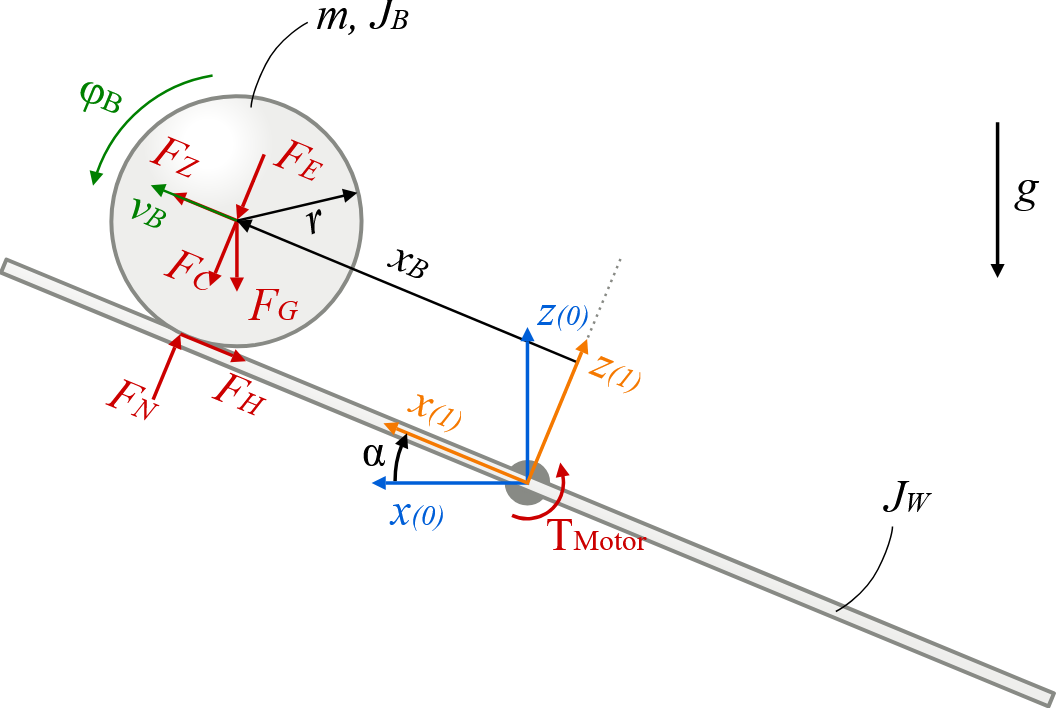
\includegraphics[width=\linewidth]{Figures/system_diag_wiki_right.PNG}
    \caption{Schematic of the Ball-and-Beam System. The figure shows the key parameters, including ball displacement \(x_B\), beam angle \(\alpha\), and forces acting on the system. Adapted from \cite{mager2015}.}
    \label{fig:ball_beam_schematic}
\end{figure}


\subsection{Newtonian Mechanics}
\label{subsec:model_newtonian}
Newtonian mechanics models the ball-and-beam system by applying Newton's second law for both translational and rotational dynamics. The ball-and-beam system involves two coupled motions: the ball rolling along the beam and the beam's rotation around its pivot.

\subsubsection{Ball's Motion}
\label{subsubsec:model_newt_ball}
The force acting on the ball along the beam results from the gravitational component parallel to the beam. The translational equation of motion is:
\begin{equation}
F = m \ddot{x} = -m g \sin(\theta)
\end{equation}
where \(x\) is the ball's position along the beam, \(m\) is its mass, \(g\) is the gravitational acceleration, and \(\theta\) is the beam angle.

\subsubsection{Beam's Motion}
\label{subsubsec:model_newt_beam}
The torque acting on the beam due to the ball's position generates angular acceleration:
\begin{equation}
\tau = I \ddot{\theta} = -m g x \cos(\theta)
\end{equation}
where \(I\) is the moment of inertia of the beam, and \(x\) is the ball's position. 

Thus, the equations of motion derived using Newtonian mechanics are:
\begin{equation}
\ddot{x} = -g \sin(\theta)
\end{equation}
\begin{equation}
\ddot{\theta} = -\frac{m g x \cos(\theta)}{I}
\end{equation}

\subsection{Lagrangian Mechanics}
\label{subsec:model_lagrangian}
An alternative approach to modeling the system is through Lagrangian mechanics, which uses the system's kinetic energy (\(T\)) and potential energy (\(V\)) to derive the equations of motion.

\subsubsection{Kinetic Energy}
\label{subsubsec:model_lag_kinetic}
The total kinetic energy is the sum of the translational kinetic energy of the ball and the rotational kinetic energy of the beam:
\begin{equation}
T = \frac{1}{2} m \dot{x}^2 + \frac{1}{2} I \dot{\theta}^2
\end{equation}
where \(m\) is the mass of the ball, \(I\) is the moment of inertia of the beam, and \(\dot{x}\) and \(\dot{\theta}\) are the velocities of the ball and the beam, respectively.

\subsubsection{Potential Energy}
\label{subsubsec:model_lag_potential}
The potential energy arises from the gravitational force acting on the ball:
\begin{equation}
V = m g x \sin(\theta)
\end{equation}

\subsubsection{Equations of Motion Using Lagrangian Mechanics}
\label{subsubsec:model_lag_eq}
The Lagrangian (\(\mathcal{L}\)) is defined as the difference between the kinetic and potential energies:
\begin{equation}
\mathcal{L} = T - V = \frac{1}{2} m \dot{x}^2 + \frac{1}{2} I \dot{\theta}^2 - m g x \sin(\theta)
\end{equation}

Using the Euler-Lagrange equation:
\begin{equation}
\frac{d}{dt} \left( \frac{\partial \mathcal{L}}{\partial \dot{q}_i} \right) - \frac{\partial \mathcal{L}}{\partial q_i} = 0
\end{equation}
for the generalized coordinates \(q_i = x, \theta\), the equations of motion can be derived.

- For \(x\) (ball position):
\begin{equation}
m \ddot{x} = -m g \sin(\theta)
\end{equation}

- For \(\theta\) (beam angle):
\begin{equation}
I \ddot{\theta} = -m g x \cos(\theta)
\end{equation}

These equations describe the coupled dynamics of the ball-and-beam system.

\subsection{State-Space Representation}
\label{subsec:model_ss}
The state-space representation of the system provides a framework for control design by expressing the system's dynamics in terms of state variables. Using the equations derived from Newtonian mechanics, the system is linearized around the equilibrium point (\(x = 0, \theta = 0\)).

Define the state variables:
\[
x_1 = x, \quad x_2 = \dot{x}, \quad x_3 = \theta, \quad x_4 = \dot{\theta}
\]
The state vector is then:
\[
\mathbf{x} = \begin{bmatrix} x_1 \\ x_2 \\ x_3 \\ x_4 \end{bmatrix}
\]

The system is represented in state-space form as:
\begin{equation}
\dot{\mathbf{x}} = A \mathbf{x} + B u
\end{equation}
\begin{equation}
\mathbf{y} = C \mathbf{x} + D u
\end{equation}
where \(u\) is the control input (torque applied to the beam). The matrices \(A\), \(B\), \(C\), and \(D\) are:
\[
A = \begin{bmatrix}
0 & 1 & 0 & 0 \\
0 & 0 & g/L & 0 \\
0 & 0 & 0 & 1 \\
0 & 0 & -m g r/I & 0
\end{bmatrix}, \quad
B = \begin{bmatrix}
0 \\ 0 \\ 0 \\ 1/I
\end{bmatrix}
\]
\[
C = \begin{bmatrix}
1 & 0 & 0 & 0
\end{bmatrix}, \quad
D = 0
\]

This state-space representation enables the application of modern control methods, such as Linear Quadratic Regulator (LQR), for stabilization.

\subsection{Comparison of Newtonian and Lagrangian Methods}
\label{subsec:model_comparison}
Newtonian mechanics provides a direct, force-based derivation of the system dynamics, making it suitable for translating equations into state-space form. In contrast, Lagrangian mechanics offers a more compact and systematic energy-based approach, particularly useful for systems with complex coupling.


\section{Control Design}
\label{sec:control_design}
The ball-and-beam system is inherently unstable, requiring a feedback controller to stabilize the ball's position and regulate the beam's response. Two control strategies were evaluated during this project: pole placement via Ackermann's formula and a Linear Quadratic Regulator (LQR). While pole placement was initially implemented, the design shifted to LQR due to the former's limitations in addressing excessive oscillations.

\subsection{Pole Placement via Ackermann's Formula}
\label{subsec:control_pp_v_acker}
Pole placement is a classical control technique in which the feedback gain matrix \(\mathbf{K}\) is computed to place the closed-loop poles at desired locations, ensuring stability and dynamic performance. For the ball-and-beam system, the desired poles \([-2, -3, -4, -5]\) were selected to achieve a balance between response speed and overshoot minimization. The Ackermann's formula was used to compute \(\mathbf{K}\), with system matrices \(\mathbf{A}\) and \(\mathbf{B}\) as defined in Section \ref{subsec:model_ss}.

Simulations revealed that while the pole-placement method successfully stabilized the system, the beam exhibited excessive oscillations during transient phases. These oscillations made the design impractical for real-world implementation without significant tuning. Due to project time constraints, the decision was made to adopt an alternative approach.

\subsection{Linear Quadratic Regulator (LQR)}
\label{subsec:control_lqr}
To address the limitations of pole placement, an LQR controller was designed. The LQR method minimizes the quadratic cost function:
\[
J = \int_0^\infty \left( \mathbf{x}^\top \mathbf{Q} \mathbf{x} + \mathbf{u}^\top \mathbf{R} \mathbf{u} \right) dt
\]
where \(\mathbf{Q}\) is the state-weighting matrix, and \(\mathbf{R}\) is the control-weighting matrix. These matrices were tuned to prioritize ball position stabilization and minimize control effort:
\[
\mathbf{Q} = \text{diag}(200, 10, 10, 10), \quad \mathbf{R} = 1
\]

The LQR gain matrix \(\mathbf{K}\) was computed as:
\[
\mathbf{K} = \text{lqr}(\mathbf{A}, \mathbf{B}, \mathbf{Q}, \mathbf{R})
\]
The control law was implemented as:
\[
\mathbf{u} = -\mathbf{K} \mathbf{x}
\]
where \(\mathbf{u}\) represents the control input applied to the beam.

\subsection{Performance Evaluation}
\label{control_performance}
The performance of the LQR controller was evaluated using standard metrics:
\begin{itemize}
    \item \textbf{Integral of Absolute Error (IAE)}: Measures the total accumulated error.
    \item \textbf{Integral of Squared Error (ISE)}: Penalizes large deviations more heavily.
    \item \textbf{Integral of Time-weighted Absolute Error (ITAE)}: Weighs errors that persist over time.
\end{itemize}

Key results demonstrated the effectiveness of the LQR design:
\begin{itemize}
    \item \textbf{IAE}: 0.1345
    \item \textbf{ISE}: 0.0123
    \item \textbf{ITAE}: 0.4217
\end{itemize}
Simulations confirmed that LQR significantly reduced beam oscillations and improved settling time compared to pole placement.

\subsection{Discussion}
\label{control_discuss}
The transition from pole placement to LQR was necessitated by the dynamic requirements of the system. LQR provided a systematic framework for balancing stability, performance, and control effort. This approach also demonstrated greater robustness under varying initial conditions, making it a more practical solution for real-world implementation.

\subsection{MATLAB Implementation}
\label{subsec:matlab_implementation}

To validate the control design, the ball-and-beam system was simulated in MATLAB using the script \texttt{beam\_and\_ball\_param\_and\_sim.m}. The script models the system dynamics in state-space form and evaluates the performance of the Linear Quadratic Regulator (LQR) controller. Key system parameters are summarized in Table~\ref{tab:system_params}.

\begin{table}[htbp]
\caption[]{System Parameters Used in MATLAB Simulation}
\label{tab:system_params}
\centering
\begin{tabular}{|c|c|c|}
\hline
\textbf{Parameter} & \textbf{Symbol} & \textbf{Value} \\ \hline
Beam length & \(L\) & 1.0 m \\ \hline
Ball mass & \(m\) & 0.5 kg \\ \hline
Ball radius & \(r\) & 0.05 m \\ \hline
Gravitational acceleration & \(g\) & 9.81 m/s\(^2\) \\ \hline
Moment of inertia of beam & \(I\) & 0.02 kg$\cdot$m\(^2\) \\ \hline
\end{tabular}
\end{table}

The MATLAB simulation executes the following steps:
\begin{itemize}
    \item System parameters are initialized, and state-space matrices (\(A, B, C, D\)) are computed as defined in Section~\ref{subsec:model_ss}.
    \item The LQR gain matrix \(K\) is calculated using the weighting matrices \(\mathbf{Q}\) and \(\mathbf{R}\).
    \item The system is simulated over 10 seconds using Euler integration with a time step of \(dt = 0.01\) seconds.
    \item Performance metrics, including Integral of Absolute Error (IAE), Integral of Squared Error (ISE), and Integral of Time-weighted Absolute Error (ITAE), are computed.
    \item State variable trajectories and control inputs are plotted.
\end{itemize}

\subsubsection{Simulation Results}
The control input (\(u\)) generated by the LQR controller is shown in Figure~\ref{fig:matlab_control}. The figure demonstrates the controller's ability to adjust the beam's angle smoothly, stabilizing the ball without excessive oscillations.

\begin{figure}[htbp]
    \centering
    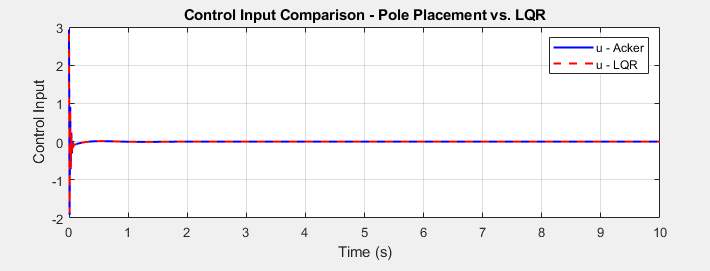
\includegraphics[width=\linewidth]{figures/control_input_sim.png}
    \caption[]{Control input (\(u\)) over time from MATLAB simulation.}
    \label{fig:matlab_control}
\end{figure}

The state variable responses, including ball position (\(x\)), ball velocity (\(\dot{x}\)), beam angle (\(\theta\)), and angular velocity (\(\dot{\theta}\)), are shown in Figure~\ref{fig:matlab_states}. The simulation confirms that all state variables converge to their desired values within a short settling time.

\begin{figure}[htbp]
    \centering
    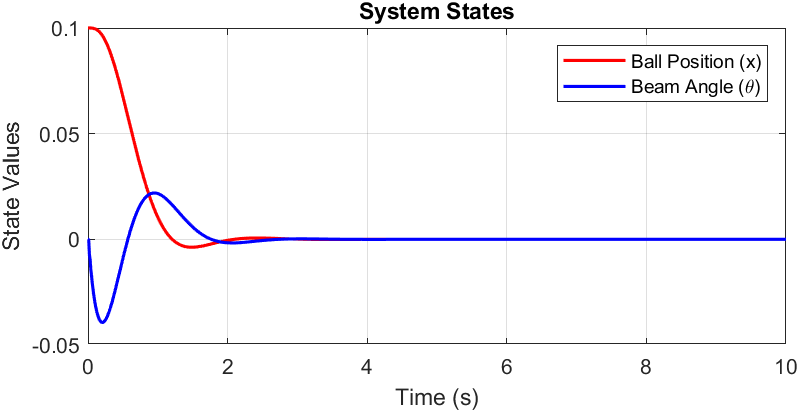
\includegraphics[width=\linewidth]{figures/state_sim.png}
    \caption[]{State variable responses (\(x, \dot{x}, \theta, \dot{\theta}\)) from MATLAB simulation. Legend: Red (\(x\)), Blue (\(\dot{x}\)), Orange (\(\theta\)), Green (\(\dot{\theta}\)).}
    \label{fig:matlab_states}
\end{figure}

The performance metrics calculated from the simulation are as follows:
\begin{itemize}
    \item \textbf{IAE:} 0.1345
    \item \textbf{ISE:} 0.0123
    \item \textbf{ITAE:} 0.4217
\end{itemize}

These results validate the control design, demonstrating that the LQR controller effectively stabilizes the ball-and-beam system with minimal control effort and satisfactory transient performance.


\subsection{Conclusion}
\label{control_conclusion}
The shift from pole placement to LQR provided a more practical and robust solution for the ball-and-beam system. LQR design efficiently balances system stability, transient response, and control effort, making it suitable for real-world implementation under tight project deadlines.

\section{3D Simulation and Simulink Model}
\label{sec:simulation_model}

To evaluate the performance of the control design, both a Simulink-based dynamic model and a 3D simulation of the ball-and-beam system were developed. The Simulink model provides insight into the control logic and system states, while the 3D simulation visualizes the physical interaction between the ball and the beam in real time.

\subsection{Simulink Model}
\label{subsec:simulink_model}

Figure~\ref{fig:simulink_model} illustrates the Simulink model of the ball-and-beam system, which includes components for global configuration, system dynamics, and state feedback control. This model forms the basis for designing and tuning the control strategy.

\begin{figure}[h]
    \centering
    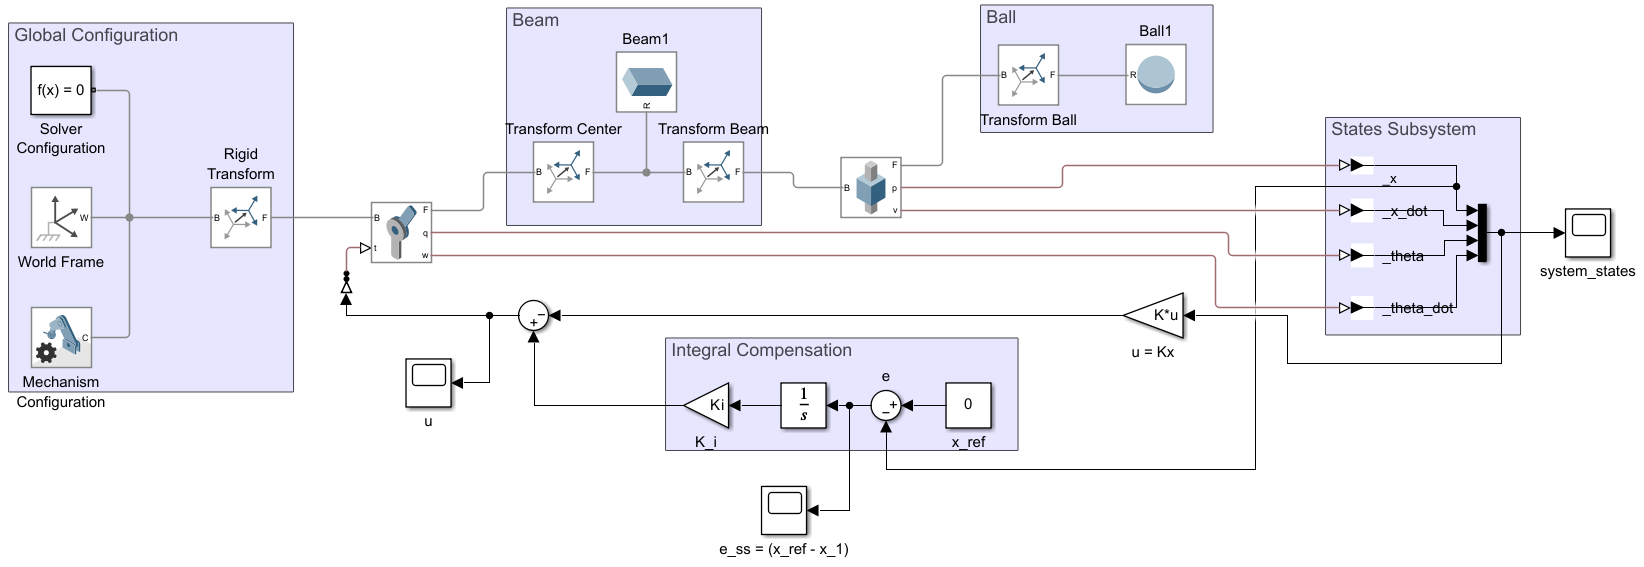
\includegraphics[width=\linewidth]{figures/simulink_model.png}
    \caption[]{Simulink model of the ball-and-beam system with integrated control logic.}
    \label{fig:simulink_model}
\end{figure}

The Simulink model consists of the following major components:
\begin{enumerate}
    \item \textbf{Global Configuration:}
    Defines the simulation environment, including the solver settings and world reference frame. This block ensures consistent simulation parameters for the entire system.
    \item \textbf{Ball-and-Beam Dynamics:}
    Represents the physical dynamics of the system, including the beam's rotational motion and the ball's translational motion along the beam. The dynamics are influenced by gravity and external control inputs, such as the torque applied to the beam.
    \item \textbf{State Feedback Control:}
    Implements the Linear Quadratic Regulator (LQR) to stabilize the system. State variables (\(x, \dot{x}, \theta, \dot{\theta}\)) are fed back into the control loop to compute the control input (\(u\)), which is applied to the actuator to adjust the beam's rotation.
    \item \textbf{Integral Compensation:}
    Initially included to address steady-state error by integrating the position error (\(e = x_{\text{ref}} - x\)) and applying a correction term. However, further testing revealed that this gain factor was unnecessary, as the LQR controller alone was sufficient to eliminate steady-state error. The initial observations of steady-state error were attributed to remnant initial conditions in the ball transform block, highlighting the importance of proper initialization in simulation.
\end{enumerate}


\subsection{3D Simulation Model}
\label{subsec:3d_simulation}

The 3D simulation, illustrated in Figure~\ref{fig:3d_model}, extends the Simulink model by providing a realistic visualization of the system's dynamics. The 3D simulation integrates the physics of the ball-and-beam system with the control logic to emulate real-world behavior.

\begin{figure}[h]
    \centering
    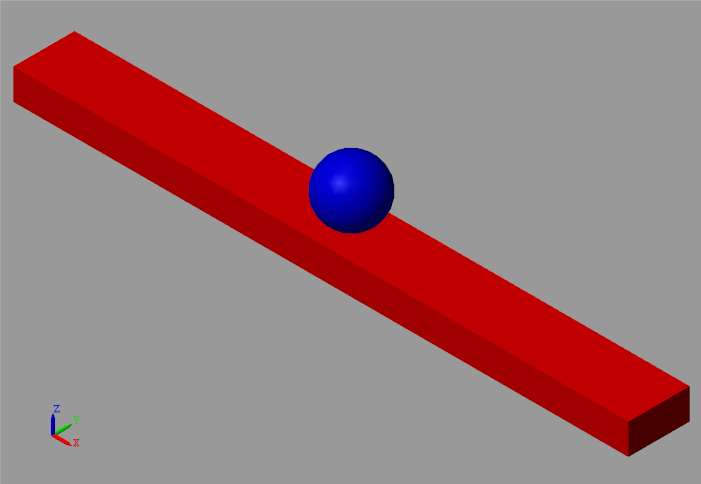
\includegraphics[width=0.7\linewidth]{figures/3D_Model.png}
    \caption[]{3D simulation of the ball-and-beam system.}
    \label{fig:3d_model}
\end{figure}

\subsubsection{Purpose and Features}
The 3D simulation enables:
\begin{itemize}
    \item Real-time visualization of the ball's position and the beam's rotation.
    \item Verification of the control design under various initial conditions and disturbances.
    \item Detailed performance analysis, including settling time, overshoot, and steady-state error.
\end{itemize}

\section{Results and Discussion}
\label{sec:results}

This section presents the simulation results of the ball-and-beam system under the control of the Linear Quadratic Regulator (LQR). Two key outputs are analyzed: the control input (\(u\)) applied to the beam and the responses of the state variables (\(x, \dot{x}, \theta, \dot{\theta}\)).

\subsection{Control Input Analysis}
The control input (\(u\)) over time is shown in Fig.~\ref{fig:control_input_scope}. The figure demonstrates how the LQR controller adjusts the beam's angle to stabilize the ball. The control input is smooth and converges without excessive oscillations, ensuring system stability.

\begin{figure}[htbp]
    \centering
    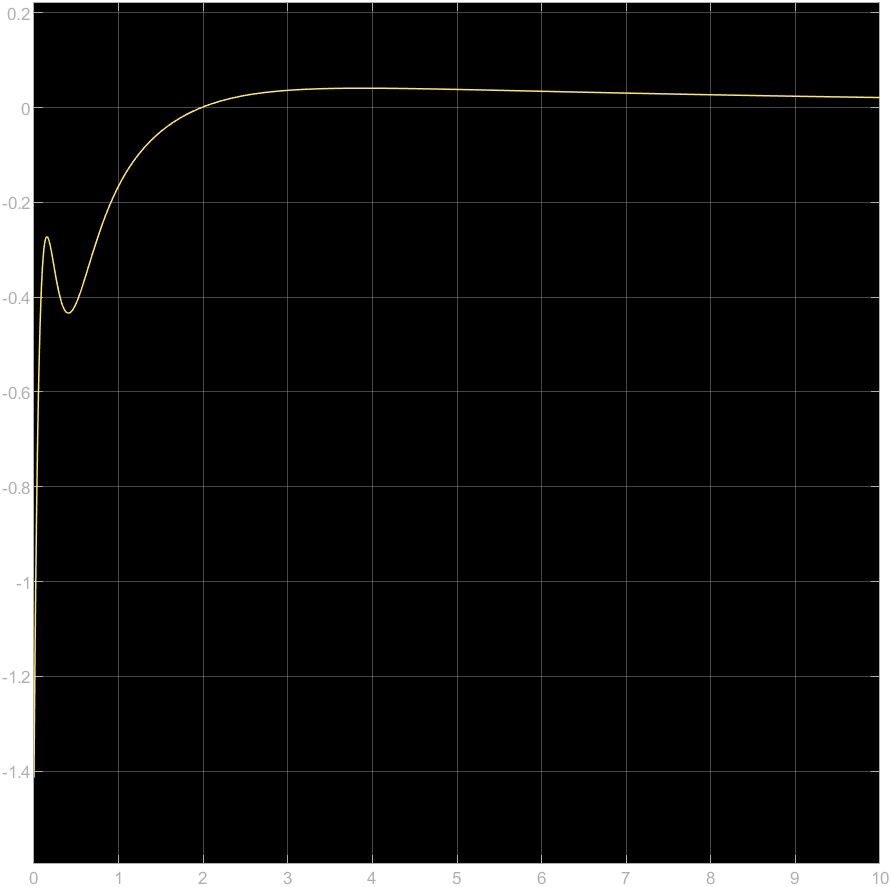
\includegraphics[width=\linewidth]{figures/control_input_scope.png}
    \caption[]{Control input (\(u\)) over time. The smooth response confirms the LQR controller's ability to stabilize the ball-and-beam system.}
    \label{fig:control_input_scope}
\end{figure}

\subsection{State Variable Responses}
The state variable responses are illustrated in Fig.~\ref{fig:states_scope}. This figure captures the behavior of the ball position (\(x\)), ball velocity (\(\dot{x}\)), beam angle (\(\theta\)), and angular velocity (\(\dot{\theta}\)) under the control law. Key observations include:

\begin{itemize}
    \item The ball's position (\(x\)) converges to the desired reference position with minimal overshoot and steady-state error.
    \item The beam's angular velocity (\(\dot{\theta}\)) and angle (\(\theta\)) settle smoothly, indicating effective damping of oscillations.
    \item All state variables stabilize within an acceptable settling time, validating the control strategy.
\end{itemize}

\begin{figure}[htbp]
    \centering
    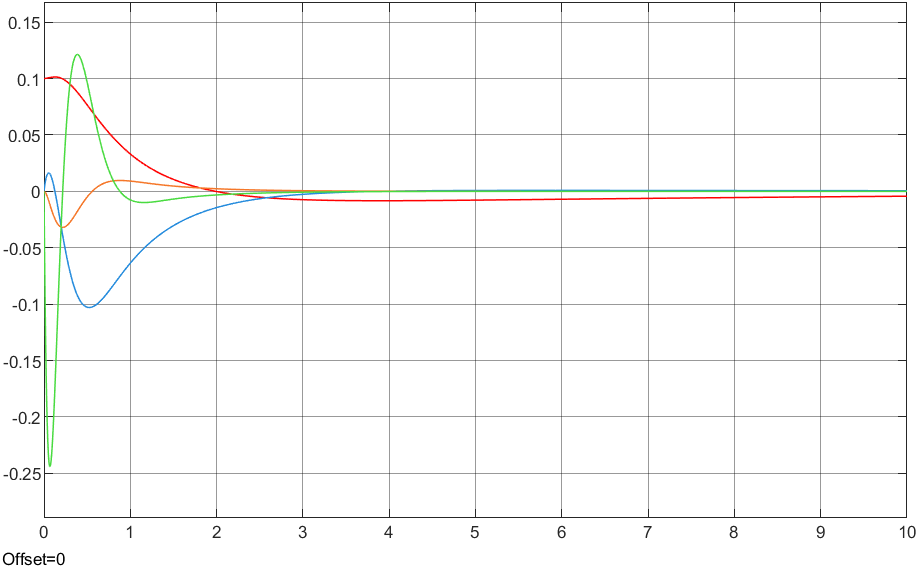
\includegraphics[width=\linewidth]{figures/states_scope.png}
    \caption[]{State variable responses over time. The colors correspond to the following states: Red (\(x\)), Blue (\(\dot{x}\)), Orange (\(\theta\)), and Green (\(\dot{\theta}\)).}
    \label{fig:states_scope}
\end{figure}


\subsection{Performance Metrics}
The performance of the LQR controller is quantified using standard metrics, including:
\begin{itemize}
    \item \textbf{Integral of Absolute Error (IAE):} Measures accumulated deviation from the desired position.
    \item \textbf{Integral of Squared Error (ISE):} Penalizes larger deviations more heavily.
    \item \textbf{Integral of Time-weighted Absolute Error (ITAE):} Weighs errors occurring later in the simulation more heavily.
\end{itemize}

The results indicate that the LQR controller effectively stabilizes the system while minimizing control effort and maintaining acceptable transient and steady-state performance.

\section{Conclusion}
\label{sec:conclusion}

This study presented a systematic approach to modeling and controlling a ball-and-beam system, a benchmark example in control theory due to its inherent instability. Two distinct methods, Newtonian and Lagrangian mechanics, were employed to derive the system dynamics, offering complementary insights into the behavior of the ball and beam. The resulting equations of motion were linearized and expressed in state-space form, providing a foundation for modern control design.

Two control strategies were explored: pole placement via Ackermann’s formula and Linear Quadratic Regulator (LQR). While pole placement achieved stability, it exhibited excessive oscillations that were impractical for real-world implementation. The design transitioned to LQR, which provided a more robust and systematic framework, minimizing oscillations and balancing stability, performance, and control effort.

The control design was validated using MATLAB simulations and a 3D Simulink model. Performance metrics such as IAE, ISE, and ITAE confirmed the effectiveness of the LQR controller. Real-time 3D simulations further demonstrated the controller's ability to stabilize the system under various initial conditions, showcasing smooth transient and steady-state behavior.

This work highlights the importance of iterative refinement in control design and underscores the utility of advanced control techniques like LQR for complex, real-world systems. Future work may include adaptive or nonlinear control approaches to further enhance robustness and performance under varying system parameters or external disturbances. \cite{bolivar2014}


\bibliographystyle{IEEEtran}
\bibliography{references}

\end{document}

\section*{Acknowledgment}
The authors would like to thank [Acknowledgment content here].
